\documentclass[11pt,a4paper]{article}

\usepackage[T1]{fontenc}
\usepackage[utf8]{inputenc}
\usepackage{lmodern}
\usepackage[margin=27mm]{geometry}
\usepackage{amsmath,amssymb,mathtools}
\usepackage{booktabs,tabularx,array}
\usepackage{tikz}
\usetikzlibrary{arrows.meta,positioning}
\usepackage[hidelinks]{hyperref}
\usepackage{microtype}

\newcommand{\R}{\mathbb{R}}
\newcommand{\LN}{\operatorname{LN}}
\newcommand{\GN}{\operatorname{GN}}
\newcommand{\MHA}{\operatorname{MHA}}
\newcommand{\FFN}{\operatorname{FFN}}
\newcommand{\silu}{\operatorname{SiLU}}
\newcommand{\softmax}{\operatorname{softmax}}
\newcommand{\BOS}{\ensuremath{\mathrm{BOS}}}
\newcommand{\EOS}{\ensuremath{\mathrm{EOS}}}
\newcommand{\code}[1]{\texttt{\detokenize{#1}}}
\newcolumntype{Y}{>{\raggedright\arraybackslash}X}
\numberwithin{equation}{section}
\setlength{\parindent}{0pt}
\setlength{\parskip}{0.45em}
\setlength{\emergencystretch}{2em}
\allowdisplaybreaks[1]

\title{Causal Video-to-Text Learning\\
\large Model Architecture and Forward-Pass Sequence}
\author{}
\date{}

\begin{document}
\maketitle
\vspace{-2em}

\begin{abstract}
This document follows the inputs through the implemented model in
\code{train.py}: mouth preprocessing, visual and textual encoders, modality
projections, cross-attention, residual fusion, vocabulary prediction, and
frame confidence. It identifies the order of the blocks, their tensor
shapes, and the information exchanged between them. Both token-query and
frame-prediction variants are covered, followed by the cached execution
order used by \code{infer.py}. The companion training document~\cite{training}
defines alignment preparation, losses, confidence targets, and optimization.
\end{abstract}

\section{The complete route}
\label{sec:overview}

The model has two inputs: video frames and a preceding token sequence.
It has two neural outputs: vocabulary logits and one confidence logit per
frame. Audio is not an input to this network. During training, the text is
the teacher-forced transcript prefix; during inference, it consists of
\BOS{} followed by tokens the decoder has committed.

The encoders first run independently. The video encoder keeps one feature
vector per frame; the text encoder keeps one feature vector per token
position. Their outputs enter one \code{MixedBlock}. Its cross-attention
modules combine the modalities by taking queries from one modality and
keys and values from the other. Residual additions then combine vectors
at the \emph{query's} positions. There is no concatenation of the video
and text sequences, and no feedback from fusion into either encoder
within a forward pass.

Figure~\ref{fig:route} gives the overall sequence. The two outputs are
different branches: confidence does not multiply the vocabulary logits
or gate a neural attention layer. The inference controller uses confidence
to decide when to commit a predicted token.

\begin{figure}[p]
\centering
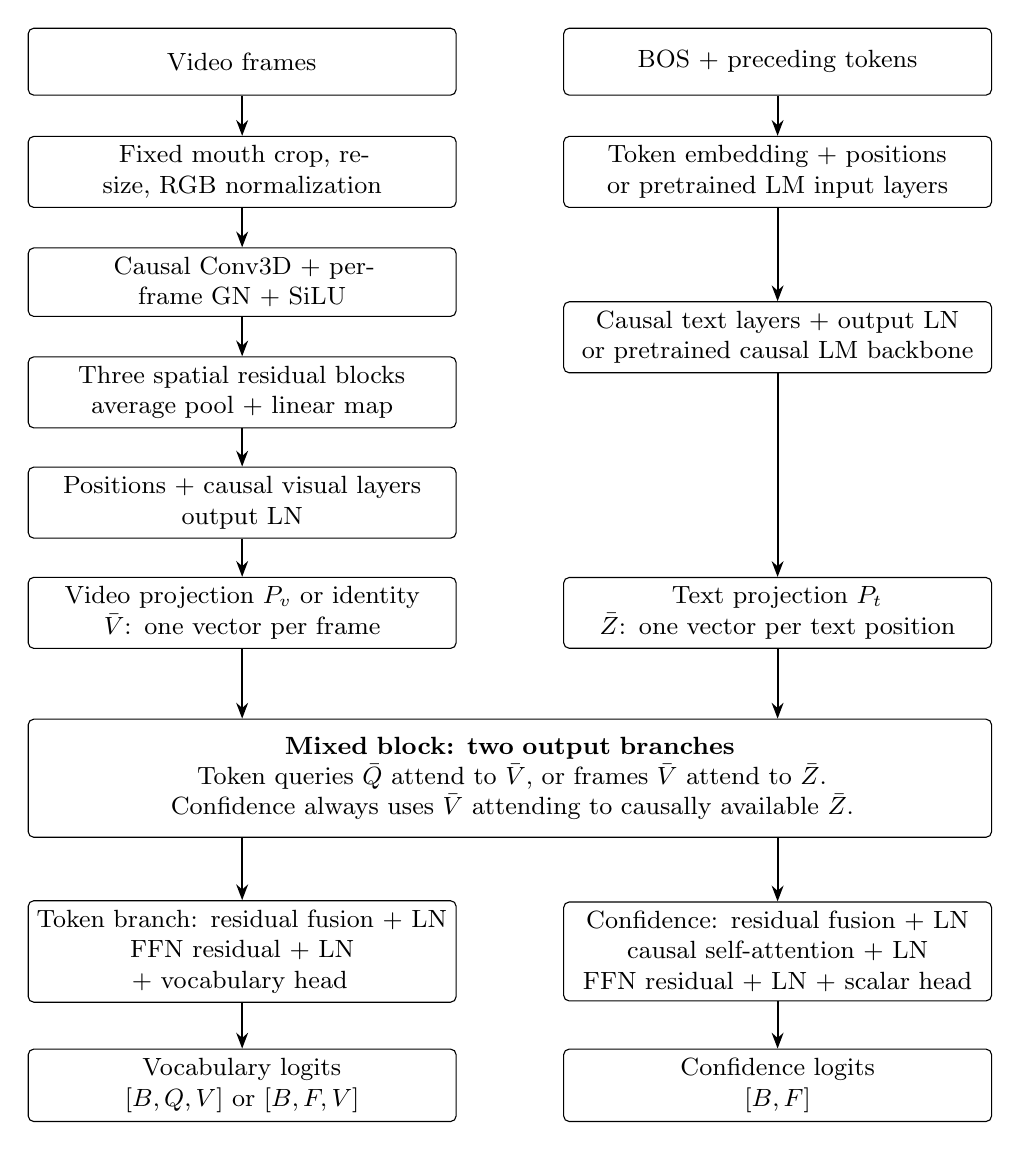
\begin{tikzpicture}[
  block/.style={draw,rounded corners=2pt,align=center,
    text width=5.2cm,minimum height=0.85cm,font=\small},
  joint/.style={block,text width=12cm,minimum height=1.5cm},
  flow/.style={-{Stealth[length=2mm]},thick}]
\node[block] (vi) at (-3.4,0) {Video frames};
\node[block] (ti) at (3.4,0) {\BOS{} + preceding tokens};
\node[block] (crop) at (-3.4,-1.4)
  {Fixed mouth crop, resize, RGB normalization};
\node[block] (emb) at (3.4,-1.4)
  {Token embedding + positions\\or pretrained LM input layers};
\node[block] (front) at (-3.4,-2.8)
  {Causal Conv3D + per-frame GN + SiLU};
\node[block] (text) at (3.4,-3.5)
  {Causal text layers + output LN\\or pretrained causal LM backbone};
\node[block] (spatial) at (-3.4,-4.2)
  {Three spatial residual blocks\\average pool + linear map};
\node[block] (temporal) at (-3.4,-5.6)
  {Positions + causal visual layers\\output LN};
\node[block] (vp) at (-3.4,-7)
  {Video projection $P_v$ or identity\\$\bar V$: one vector per frame};
\node[block] (tp) at (3.4,-7)
  {Text projection $P_t$\\$\bar Z$: one vector per text position};
\node[joint] (mix) at (0,-9.1)
  {\textbf{Mixed block: two output branches}\\
   Token queries $\bar Q$ attend to $\bar V$, or frames $\bar V$ attend to $\bar Z$.\\
   Confidence always uses $\bar V$ attending to causally available $\bar Z$.};
\node[block] (token) at (-3.4,-11.3)
  {Token branch: residual fusion + LN\\FFN residual + LN + vocabulary head};
\node[block] (conf) at (3.4,-11.3)
  {Confidence: residual fusion + LN\\causal self-attention + LN\\FFN residual + LN + scalar head};
\node[block] (yo) at (-3.4,-13)
  {Vocabulary logits\\$[B,Q,V]$ or $[B,F,V]$};
\node[block] (co) at (3.4,-13)
  {Confidence logits\\$[B,F]$};
\draw[flow] (vi) -- (crop);
\draw[flow] (crop) -- (front);
\draw[flow] (front) -- (spatial);
\draw[flow] (spatial) -- (temporal);
\draw[flow] (temporal) -- (vp);
\draw[flow] (ti) -- (emb);
\draw[flow] (emb) -- (text);
\draw[flow] (text) -- (tp);
\draw[flow] (vp.south) -- (vp.south |- mix.north);
\draw[flow] (tp.south) -- (tp.south |- mix.north);
\draw[flow] (token.north |- mix.south) -- (token.north);
\draw[flow] (conf.north |- mix.south) -- (conf.north);
\draw[flow] (token) -- (yo);
\draw[flow] (conf) -- (co);
\end{tikzpicture}
\caption{Order of the model blocks. Cross-attention visibility is governed
by Section~\ref{sec:masks}. The detailed additions inside the mixed block
are given in Sections~\ref{sec:token}--\ref{sec:confidence}.}
\label{fig:route}
\end{figure}

\section{Inputs, positions, and tensor shapes}
\label{sec:inputs}

Let $B$ be batch size, $F$ the padded number of frames, $T$ the padded
teacher-sequence length, $Q$ the padded number of selected prediction
queries, and $V$ the vocabulary size. Feature widths are $d_v$ for video,
$d_t$ for text, and $d$ inside fusion. A full video with $N$ transcript
tokens has $T=Q=N+1$, counting \BOS{} as an input position and \EOS{} as
the final token-query target. Video sections can retain a longer teacher
history than their selected queries, so $T$ and $Q$ need not be equal.

\begin{center}
\small
\begin{tabularx}{\linewidth}{@{}l l Y@{}}
\toprule
Quantity & Shape & Meaning \\
\midrule
Normalized video & $[B,F,3,S,S]$ & $S\times S$ RGB mouth crops. \\
Teacher token IDs & $[B,T]$ & \BOS{} and transcript/history IDs. \\
Encoded video $V_e$ & $[B,F,d_v]$ & Causal visual states $v_f$. \\
Encoded text $Z$ & $[B,T,d_t]$ & Causal text states $z_j$. \\
Projected video $\bar V$ & $[B,F,d]$ & Video keys/values or frame queries. \\
Projected text $\bar Z$ & $[B,T,d]$ & Text keys/values. \\
Selected text $\bar Q$ & $[B,Q,d]$ & Queries for the token-query branch. \\
Token-query logits & $[B,Q,V]$ & One distribution per selected prefix. \\
Frame-token logits & $[B,F,V]$ & One distribution per frame. \\
Confidence logits & $[B,F]$ & One scalar per frame in every variant. \\
\bottomrule
\end{tabularx}
\end{center}

Video lengths, text lengths, target endpoints, and text-availability
times are additional metadata. They construct masks and select queries;
they are not embedded as learned feature inputs. Padding can have
computed activations but is excluded as an attention key and from
supervision. The equations below suppress the batch dimension.

\section{Operations used inside the blocks}
\label{sec:primitives}

$\LN$ normalizes the features of each position. $\GN$ in the spatial
front end normalizes channel groups and spatial coordinates separately
for each frame. Let $\sigma$ be sigmoid, $\silu(x)=x\sigma(x)$, and
$\mathcal D_p$ denote dropout with probability $p$ in training and the
identity in evaluation. Distinct learned maps and normalizations have
independent parameters unless sharing is explicitly stated.

Every custom feed-forward block of width $d_*$ has the sequence
\begin{equation}
\FFN(x)=\mathcal D_p\!\left(
 W_2\mathcal D_p\!\left(\silu(W_1\LN(x)+b_1)\right)+b_2\right),
\end{equation}
where the hidden width is $m d_*$ and $m$ is \code{ff_mult}.
The residual addition occurs outside this block.

For $\MHA(U,K;M)$, queries come from $U$; both keys and values come
from $K$. Each head independently projects these inputs and computes
\begin{equation}
A^h_{rs}=\softmax_{s:M_{rs}=1}
 \left(\frac{\langle W_Q^hU_r+b_Q^h,
 W_K^hK_s+b_K^h\rangle}{\sqrt{d_h}}\right).
\end{equation}
Disallowed entries are zero. Each head aggregates its projected values
with $\mathcal D_p(A^h)$; the heads are concatenated and passed through
an output affine map. Thus the output has the query sequence length.
There are $H$ heads and $d_h=d_*/H$ features per head. Self-attention
uses the same sequence for queries, keys, and values. Attention weights
returned for regularization are measured before dropout.

\section{Video path: pixels to causal frame states}
\label{sec:video}

\subsection{Fixed crop and normalization}

\code{FixedMouthCropper} chooses a rectangle on the first frame, using
the largest detected face's lower-central region or a deterministic
lower-center fallback. This rectangle stays fixed for the video; it is
clipped to the current image bounds when applied. Each crop is resized
to $S\times S$, converted from OpenCV BGR to RGB, and normalized:
\begin{equation}
x_f=\operatorname{RGB}\!\left(\operatorname{Resize}_S(
\operatorname{Crop}_{I_0}(I_f))\right)/127.5-1.
\end{equation}
The output is arranged as $[B,F,3,S,S]$. Crop selection uses no future
frame, and preprocessing preserves the frame sequence.

\subsection{Causal Conv3D and per-frame spatial encoder}

\code{CausalConv3d} first transposes to $[B,3,F,S,S]$, pads four
frames on the left and two pixels on each spatial side, and applies a
bias-free $5\times5\times5$ convolution with stride $(1,2,2)$.
It then applies per-frame GN and SiLU. Temporal stride is one, so all
$F$ positions remain. The first convolution at frame $f$ reads only
$x_{f-4},\ldots,x_f$, using zeros for negative indices.

\code{FrameVisualEncoder} merges batch and frame axes and applies three
\code{Residual2D} blocks independently at each frame. A block is
\begin{align}
a&=\silu(\GN_1(\operatorname{Conv}_{3\times3,s=2}(u))),\\
b&=\GN_2(\operatorname{Conv}_{3\times3,s=1}(a)),\\
\mathcal R(u)&=\silu(b+\operatorname{Conv}_{1\times1,s=2}(u)).
\end{align}
All these convolutions are bias-free; the $3\times3$ convolutions use
one-pixel padding. The projection on the skip path matches both spatial
size and channel count. All three instantiated blocks use stride two.

For the default $S=96$ and initial channel count $32$, the route is:
\begin{center}
\small
\begin{tabularx}{\linewidth}{@{}l l Y@{}}
\toprule
Block & Output per frame & Effect \\
\midrule
Input & $3\times96\times96$ & Normalized RGB crop. \\
Causal Conv3D, GN, SiLU & $32\times48\times48$ & Local temporal and spatial features. \\
Spatial residual 1 & $64\times24\times24$ & Downsample spatially. \\
Spatial residual 2 & $96\times12\times12$ & Downsample spatially. \\
Spatial residual 3 & $128\times6\times6$ & Downsample spatially. \\
Adaptive average pool & $128$ & Average over the spatial grid. \\
Affine map & $d_v$ & Produce $r_f=W_r\operatorname{Pool}(u_f)+b_r$. \\
\bottomrule
\end{tabularx}
\end{center}
The batch/frame axes are then restored to $[B,F,d_v]$. The pooling
does not average across time. The final affine map here remains present
even when the later video fusion projection is disabled.

\subsection{Positions and temporal visual layers}

Sinusoidal positions are added once before the temporal stack:
$X_f^{(0)}=r_f+\mathrm{PE}_{d_v}(f)$. For width $d_*$, the implementation
uses $h=\lceil d_*/2\rceil$ and
\begin{equation}
\omega_k=10000^{-k/\max(1,h-1)},\qquad
\mathrm{PE}(f)_{2k}=\sin(f\omega_k),\quad
\mathrm{PE}(f)_{2k+1}=\cos(f\omega_k),
\end{equation}
retaining only coordinates below $d_*$. The same positional function is
used by the learned text encoder, at text positions instead of frames.

Each \code{CausalConformerLayer} applies these residual operations in order:
\begin{align}
U&=X+\tfrac12\FFN(X),\\
R&=U+\mathcal D_p\!\left[\MHA(\LN_a(U),\LN_a(U);M^{\rm causal})\right],\\
X^+&=R+\mathcal K(R).
\label{eq:visual-layer}
\end{align}
The attention mask allows a frame to read only itself and earlier
valid frames. The convolution module $\mathcal K$ has the exact sequence
\begin{align}
[A,B]&=\operatorname{Pointwise}_{d_v\to2d_v}(\LN_c(R)),\\
G&=A\odot\sigma(B),\\
J_f&=b_{\rm dw}+\sum_{r=0}^{k_c-1}d_r\odot G_{f-r},\\
\mathcal K(R)&=\mathcal D_p\!\left(
 \operatorname{Pointwise}_{d_v\to d_v}(\silu(J))\right).
\end{align}
The pointwise maps are $1\times1$ temporal convolutions. The GLU halves
the expanded channels back to $d_v$. The middle operation is a depthwise
temporal convolution, with $k_c-1$ zeros on the left and no future padding.
Each channel has its own temporal filter.

There is exactly one half-weighted FFN residual per visual layer,
followed by self-attention and convolution. After $L_v$ layers, a final
output normalization gives
\begin{equation}
v_f=\LN_{v,\rm enc}(X_f^{(L_v)})\in\R^{d_v}.
\end{equation}
These states are causal but are not restricted to the small convolution
window: self-attention can read the entire available visual prefix.

\section{Text path: preceding tokens to causal text states}
\label{sec:text}

\subsection{Learned text encoder}

Let $t_0=\BOS$ and $t_j=y_j$ for transcript tokens $j\geq1$.
\code{TextEncoder} starts with
\begin{equation}
Z_j^{(0)}=\operatorname{Embed}(t_j)+\mathrm{PE}_{d_t}(j).
\end{equation}
Each \code{CausalTextLayer} applies
\begin{align}
U&=Z+\mathcal D_p\!\left[
 \MHA(\LN_a(Z),\LN_a(Z);M^{\rm causal})\right],\\
Z^+&=U+\FFN(U).
\end{align}
After $L_t$ layers, the encoder returns
$z_j=\LN_{t,\rm enc}(Z_j^{(L_t)})$.
In particular, $z_j$ encodes only $(\BOS,y_1,\ldots,y_j)$.
The query predicting $y_i$ is $q_i=z_{i-1}$, so its own target token is
absent from that query. A full video's additional \EOS{} query uses $z_N$.

\subsection{Pretrained causal language model alternative}

With \code{--pretrained-lm}, \code{PretrainedLMTextEncoder} replaces
the entire learned text encoder by the imported causal LM backbone.
It retains that model's embedding, layers, positional mechanism, and
output normalization. Its final hidden states become $z_j$; CESM does
not add the custom text layers or sinusoidal positions afterward.
The imported vocabulary head is discarded. The mixed block's own
vocabulary head remains responsible for prediction.

The tokenizer and $d_t$ come from the imported model. A frozen backbone
runs deterministically; optional fine-tuning changes which parameters
learn, not the connection to the mixed block.

\section{Projections and causal connections}
\label{sec:masks}

\subsection{Matching feature widths}

The mixed block first puts the modalities in a common feature space:
\begin{equation}
\bar v_f=P_vv_f,\qquad \bar z_j=P_tz_j,\qquad \bar q_i=P_tq_i.
\end{equation}
By default, $d=d_{\rm fusion}$ and both projections are bias-free
linear maps. With \code{--no-vproj}, $P_v$ is the identity,
$d=d_v$, and $P_t$ maps $d_t$ to $d_v$. Every mixed-block attention,
normalization, FFN, and output head uses this effective width $d$.
The internal attention projections still operate when $P_v$ is bypassed.

\subsection{Which positions may communicate}

For inclusive alignment window $[a_i,e_i]$, token query $q_i$ reads
video keys through its endpoint:
\begin{equation}
M^{t\to v}_{if}=\mathbf1\{0\leq f\leq e_i\}.
\label{eq:t2v}
\end{equation}
This includes frames before $a_i$; the mask does not restrict attention
to the current token window. An optional training penalty encourages
window-local mass~\cite{training}.

In the reverse direction, the text state for $y_j$ becomes available
only after its aligned window has ended:
\begin{equation}
\alpha_0=0,\qquad \alpha_j=e_j+1\ (j\geq1),\qquad
M^{v\to t}_{fj}=\mathbf1\{\alpha_j\leq f\}.
\label{eq:v2t}
\end{equation}
Both cross-attention masks also enforce valid query and key positions.
All custom self-attention uses $M^{\rm causal}_{rs}=\mathbf1\{s\leq r\}$
with padded keys removed.

For example, with windows $[0,2]$ and $[3,5]$, frames $0,1,2$ may read
only $z_0$ (\BOS). Frames $3,4,5$ may also read $z_1$, which includes
the first token. They cannot read $z_2$, which becomes available at
frame $6$. The query for the second token is $z_1$ and may read video
frames $0$ through $5$ when evaluated at its training endpoint.

\section{Token-query prediction branch}
\label{sec:token}

This branch is used by \code{residual}, \code{cross_only}, and
\code{weighted} fusion. After selecting $q_i=z_{i-1}$, its sequence is
\begin{align}
c_i&=\MHA_{t\to v}(\bar Q,\bar V;M^{t\to v})_i,
 &&\text{\code{text_cross}},\\
h_i&=\LN_t(\rho\bar q_i+c_i),
 &&\text{\code{text_ln}},\\
\widehat h_i&=\LN_{t,\rm out}(h_i+\FFN_t(h_i)),
 &&\text{\code{text_ffn}, \code{text_ffn_ln}},\\
\ell_i&=W_y\widehat h_i+b_y,
 &&\text{\code{token_head}}.
\label{eq:token-path}
\end{align}
Here $\rho=1$ for residual fusion, $\rho=0$ for cross-only fusion, and
$\rho=w_t$ for weighted fusion. The configurable $w_t$ is a fixed
finite scalar, not an optimized parameter. The combination is addition
at each query position, and the output logits have shape $[B,Q,V]$.

The residual and attention output are normalized \emph{after} their
addition. Cross-attention itself receives the projected encoder states
directly. The FFN has its own input LN and a second residual addition,
followed by the separate output LN shown above.

Removing the direct text residual does not remove text conditioning:
the attention queries still depend on $\bar q_i$. Likewise, weighted
fusion with $w_t=0$ reproduces the cross-only combination. The norm-margin
experiment on \code{tcross} changes a loss, leaving this forward path
unchanged. The scalar confidence branch is separate from these logits.

\section{Frame-token prediction branch}
\label{sec:frame}

With \code{text_fusion=frame}, frames become the vocabulary prediction
positions. There is no \code{text_cross} module. The full teacher-state
sequence supplies the causally available text keys and values:
\begin{align}
d_f&=\MHA_{v\to t}(\bar V,\bar Z;M^{v\to t})_f,
 &&\text{\code{video_cross}},\\
h_f^{\rm fr}&=\LN_t(\bar v_f+w_vd_f),
 &&\text{\code{text_ln}},\\
\widehat h_f^{\rm fr}&=\LN_{t,\rm out}
 (h_f^{\rm fr}+\FFN_t(h_f^{\rm fr})),\\
\ell_f^{\rm fr}&=W_y\widehat h_f^{\rm fr}+b_y.
\label{eq:frame-path}
\end{align}
The final two operations use \code{text_ffn}, \code{text_ffn_ln}, and
\code{token_head}, despite the frame indexing. Their logits have shape
$[B,F,V]$. The fixed finite scalar $w_v$ is
\code{frame_vcross_weight}, set by \code{--vcross-weight}, and defaults
to one. At $w_v=0$, these token logits depend only on visual features.

\code{video_cross} also supplies the attention operation in the
confidence branch. It shares parameters across the two uses, but the
confidence residual always adds $d_f$ with coefficient one. Separate
batched calls can draw different dropout masks during training; streaming
evaluation computes $d_f$ once for both outputs. The token branch does
not pass through the confidence branch's causal self-attention or FFN.

Frames inside real-token windows receive training labels; gaps, padding,
and \EOS{} do not receive frame labels. Window phasing adds a previous-token
loss on selected frames, using the same blocks with a stricter text mask that
excludes that previous token and all later text. Encoder outputs and projected
queries, keys, and values are shared between the two paths~\cite{training}.

\section{Confidence branch in every variant}
\label{sec:confidence}

The confidence branch operates on the frame sequence and uses the
full causally available text history. Its exact order is
\begin{align}
d_f&=\MHA_{v\to t}(\bar V,\bar Z;M^{v\to t})_f,
 &&\text{\code{video_cross}},\\
g_f&=\LN_v(\bar v_f+d_f),
 &&\text{\code{video_ln}},\\
s_f&=\MHA_{v,\rm self}(\LN_a(G),\LN_a(G);M^{\rm causal})_f,
 &&\text{\code{video_self_norm}, \code{video_self}},\\
g'_f&=\LN_{v,\rm self}(g_f+s_f),
 &&\text{\code{video_self_ln}},\\
\widehat g_f&=\LN_{v,\rm out}(g'_f+\FFN_v(g'_f)),
 &&\text{\code{video_ffn}, \code{video_ffn_ln}},\\
\kappa_f&=w_c^{\mathsf T}\widehat g_f+b_c,
 &&\text{\code{conf_head}}.
\label{eq:confidence-path}
\end{align}
Here $G$ is the sequence of $g_f$ states. The confidence self-attention
lets the current fused frame state read earlier fused frame states;
it is distinct from self-attention in the video encoder. The final
singleton feature axis is squeezed, yielding $[B,F]$ logits.

Probabilities are formed outside the model heads:
\begin{equation}
p=\softmax(\ell/\tau_y),\qquad C_f=\sigma(\kappa_f/\tau_c),
\qquad \tau_y,\tau_c>0.
\end{equation}
Stage-I cross entropy uses the raw vocabulary logits. Confidence-target
construction and inference use their configured temperatures. Confidence
is trained to reflect predictive certainty and stability, rather than
being a direct estimate of token correctness; its target construction
is defined in the training document~\cite{training}.

\section{Execution order: batch training and a live sequence}
\label{sec:execution}

\subsection{Which branches are evaluated during training}

\code{UnnobaModel.forward} encodes video and teacher text first. In
token-query variants, \code{select_text_queries} selects the supervised
prefix states. The mixed block's \code{forward_token} method then evaluates
Section~\ref{sec:token}. Frame mode passes the full teacher states to
\code{forward_frame}, which evaluates Section~\ref{sec:frame}. The standard
Stage-I call returns vocabulary logits and representation/attention
data for its losses; it does not compute confidence logits.

\code{UnnobaModel.forward_confidence} evaluates the confidence branch
in Stage II (Section~\ref{sec:confidence}). Its targets come from the
frozen prediction path. The encoders, projections, and vocabulary
path are frozen. Confidence-only layers train; \code{video_cross} also
trains in token-query variants, but stays frozen in frame mode because
it participates in frame-token prediction. These are execution and
parameter-selection differences, not additional neural blocks.

If training splits a video into sections, visual history and visual
positions restart at each section. The original fixed crop and preceding
text prefix are retained. Availability times and query selection are
translated to the section's coordinates as specified in
\cite{training}; sectioned visual context can therefore differ from an
uninterrupted inference stream.

\subsection{Streaming one frame at a time}

The main loop in \code{infer.py} uses this order:
\begin{enumerate}
\item Initialize empty caches, then call \code{stream_push_text_token}
  with \BOS. This encodes the token, applies $P_t$, appends its
  keys/values to \code{video_cross}, and saves it as the current text query.
\item Read and preprocess frame $f$. \code{stream_push_video_frame}
  applies the visual blocks in Section~\ref{sec:video} using cached past
  context, then applies $P_v$.
\item In token-query variants, append this projected frame's keys/values
  to \code{text_cross}. In every variant, let the frame query the currently
  committed text via \code{video_cross}; evaluate the confidence branch.
  Frame mode also computes and stores its frame-token logits at this step.
\item Call \code{stream_predict_next}. In token-query variants, the saved
  text query attends to all video keys now cached, and the token head
  produces the next-token logits. Frame mode returns the stored logits
  from the latest video step.
\item The inference controller masks non-generatable special IDs,
  applies temperature and softmax, and selects the most probable token.
  It uses the candidate's accumulated peak confidence together with
  warmup, minimum-gap, repeat-cooldown, probability, and stability guards
  to decide whether to commit it.
\item If a normal token is committed, append that ID to the text encoder,
  project its new state, extend the text keys/values, and replace the
  current text query. This text becomes visible to the next frame's
  video-to-text attention. A committed \EOS{} ends decoding. Otherwise
  keep the current prefix and advance to the next frame.
\end{enumerate}

Appending text does not recompute earlier video or confidence states.
In frame mode it also does not recompute the stored frame-token logits;
the updated text affects frame prediction on the next video push. The
normal frame loop permits at most one commitment per processed frame.
An optional end-of-video flush is a separate controller operation.

\begin{center}
\small
\begin{tabularx}{\linewidth}{@{}l Y@{}}
\toprule
Cache & What is retained between steps \\
\midrule
Visual Conv3D & Previous four normalized input frames. \\
Each visual temporal layer & Self-attention keys/values and $k_c-1$ GLU outputs. \\
Text encoder & Self-attention keys/values, or the imported LM's native cache. \\
Text-to-video attention & Projected video keys/values; absent in frame mode. \\
Video-to-text attention & Projected committed-text keys/values. \\
Confidence self-attention & Keys/values of the normalized fused frame states. \\
Decoder state & Position counters, current text query, and frame logits in frame mode. \\
\bottomrule
\end{tabularx}
\end{center}

With dropout disabled, these cached operations evaluate the same causal
functions as masked batch computation for identical visual context and
text-commit history, up to numerical precision. Attention caches grow
with the observed sequence. Convolution caches retain only their finite
past windows. Teacher-forced and generated histories can differ in both
token identity and commitment time.

\section{Configuration reference}
\label{sec:configuration}

The following are the defaults for a fresh \code{train.py} CLI run,
not values inferred from a particular checkpoint:
\begin{center}
\small
\begin{tabularx}{\linewidth}{@{}l l Y@{}}
\toprule
Setting & Default & Role \\
\midrule
\code{--mouth-size} & $96$ & Spatial input size $S$. \\
\code{--conv3d-channels} & $32$ & Channels after the first visual convolution. \\
\code{--d-video} & $256$ & Visual encoder width $d_v$. \\
\code{--d-text} & $256$ & Learned text encoder width $d_t$. \\
\code{--d-fusion} & $256$ & Fusion width when video projection is enabled. \\
\code{--heads} & $4$ & Heads in custom attention modules. \\
\code{--video-layers} & $2$ & Number $L_v$ of temporal visual layers. \\
\code{--text-layers} & $2$ & Number $L_t$ of learned text layers. \\
\code{--ff-mult} & $1$ & FFN hidden-width multiplier $m$. \\
\code{--conv-kernel} & $7$ & Depthwise temporal kernel $k_c$. \\
\code{--dropout} & $0.1$ & Custom attention/FFN/convolution dropout. \\
Fusion mode & residual & Resolved default for a new training run. \\
Video projection & enabled & \code{--no-vproj} replaces it by identity. \\
\code{--w-t} & $1$ & Text residual weight in weighted fusion. \\
\code{--vcross-weight} & $1$ & Resolved text-attention weight in frame mode. \\
\bottomrule
\end{tabularx}
\end{center}

Constructing \code{ModelConfig} directly instead uses
\code{video_layers=4} and \code{ff_mult=4} unless overridden. Checkpoints
store the effective architecture. Custom attention widths must be
divisible by the chosen number of heads. With a pretrained LM, its own
text architecture replaces the learned-text width/layer defaults.

The five experiment scripts correspond to residual fusion, residual
fusion with a cross-output norm penalty, cross-only fusion, weighted
fusion, and frame fusion. Only the second experiment changes the loss
without changing the baseline forward graph.

\begin{thebibliography}{9}
\bibitem{training}
\emph{Causal Video-to-Text Learning: Mathematical Formulation and Training
Procedure}. Companion document, \code{train_mathematics.tex}.
\href{train_mathematics.pdf}{Compiled training document}.
\end{thebibliography}

\end{document}
